
\documentclass{article}
\usepackage[spanish]{babel} %Definir idioma español
\usepackage[utf8]{inputenc} %Codificacion utf-8
\usepackage{amssymb, amsmath, amsbsy, wasysym}
\usepackage{multirow} % para tablas
\usepackage{graphicx}
\usepackage{listings}
\title{Tarea 3\\Gráficos probabilistas}
\author{Emmanuel Peto Gutiérrez}
\begin{document}
\maketitle

\section{Ejercicio 1}

\subsection{Redes y descripción}

\textbf{Red 1.}

\begin{center}
\includegraphics[scale=1]{ej1_red1}
\end{center}

Descripción.

\begin{itemize}
\item $T$: la temperatura del reactor es independiente, pues no reacciona conforme a la alarma ni al medidor.
\item La defectuosidad de los dispositivos ($D_I$ y $D_A$) también son independientes.
\item $I$: la medida del indicador depende, evidentemente, de la temperatura real del reactor ($T$) y de su defectuosidad ($D_I$).
\item $A$: La alarma se activa solamente si el indicador de temperatura rebasa cierto umbral, así que depende de $I$. También depende de si el dispositivo de alarma funciona o no ($D_A$).
\end{itemize}

\textbf{Red 2.}

\begin{center}
\includegraphics[scale=1]{ej1_red2}
\end{center}

Descripción.

Las dependencias son casi iguales que en la primera red, excepto que la defectuosidad de los dispositivos no es independiente. En este caso, supongamos que las altas temperas del reactor daña los circuitos de los dispositivos de medición y de alarma, en ese caso la efectividad de los dispositivos ($D_I$ y $D_A$) depende de la temperatura ($T$).

\textbf{Red 3.}

\begin{center}
\includegraphics[scale=1]{ej1_red3}
\end{center}

Descripción.

En este caso, después de que suenan las alarmas, los operadores de la planta empiezan a bajar la temperatura del reactor. Por lo tanto, la temperatura se hace dependiente de la alarma.

Entre estas redes, la que tiene el mayor número de independencias condicionales es la red 3.

\subsection{Distribución conjunta}

Ahora se describe la probabilidad conjunta de cada red.

\begin{itemize}
\item \textbf{Red 1:} $P(A, I, T, D_I, D_A) = P(D_I) \cdot P(D_A) \cdot P(T) \cdot P(I | T, D_I) \cdot P(A | I, D_A)$

\item \textbf{Red 2:} $P(A, I, T, D_I, D_A) = P(T) \cdot P(D_I | T) \cdot P(D_A | T) \cdot P(I | T, D_I) \cdot P(A | I, D_A)$

\item \textbf{Red 3:} $P(A, I, T, D_I, D_A) = P(D_I) \cdot P(D_A) \cdot P(I | D_I) \cdot P(A | I, D_A) \cdot P(T | A)$

\end{itemize}

\subsection{Valores por nodo}

Ahora se calculará, para cada red, el número de valores que puede haber por cada nodo. O dicho de otra forma, el número de filas que habría en una tabla que describa la probabilidad condicional de cada nodo. Se asumen valores binarios para $D_I$, $D_A$, $A$ y 100 valores para $I$, $T$.

\textbf{Red 1}

\begin{itemize}
\item $D_I$: 2
\item $D_A$: 2
\item $T$: 100
\item $I$: $100 \times 100 \times 2 = 20000$
\item $A$: $2 \times 100 \times 2 = 400$
\item Total: 20504
\end{itemize}

\textbf{Red 2}

\begin{itemize}
\item $D_I$: $2 \times 100 = 200$
\item $D_A$: $2 \times 100 = 200$
\item $T$: 100
\item $I$: $100 \times 100 \times 2 = 20000$
\item $A$: $2 \times 100 \times 2 = 400$
\item Total: 20900
\end{itemize}

\textbf{Red 3}

\begin{itemize}
\item $D_I$: 2
\item $D_A$: 2
\item $T$: $100 \times 2 = 200$
\item $I$: $100 \times 2 = 200$
\item $A$: $2 \times 100 \times 2 = 400$
\item Total: 804
\end{itemize}

\section{Ejercicio 2}

\begin{itemize}

\item $T \perp F | D$: falso.

$T$ y $F$ no son independientes dado $D$ por el esquema de efecto común. Esto es porque la variable observada $D$ es descendiente de $T$ y también es descendiente de $F$.

\item $C \perp B | F$: verdadero.

$C$ y $B$ son independientes dado $F$ por el esquema de causa común. Esto es porque la variable observada $F$ es padre de $C$ y también es padre de $B$.

\item $A \perp F | C$: verdadero.

$A$ y $F$ son independientes por el esquema de efecto común. Esto es porque tanto $A$ como $F$ son ancestros de la variable $D$ y la variable observada $C$ no bloquea los caminos entre $A$ y $D$ ni entre $F$ y $D$.

\item $A \perp F | D, C$: falso.

$A$ y $F$ no son independientes dados $D$ y $C$ porque todos los caminos de la gráfica (no dirigida) entre $A$ y $F$ están bloqueados.

\end{itemize}

\section{Ejercicio 3}

\textbf{a) Distribución conjunta}

$P(E, F, S, V, D, C) = P(E) \cdot P(F | E) \cdot P(S | E) \cdot P(V | F, E) \cdot P(D | V) \cdot P(C | S)$\\

\textbf{b) Campo de Markov}

Se forma un clan con los padres de $V$, que son $F$ y $S$. Para el resto de las aristas simplemente se les quita la dirección.

\begin{center}
\includegraphics[scale=1]{ej3}
\end{center}

\textbf{c) Fiebre}

Supongamos que en el 100\% de los casos, las personas infectadas con ébola tienen fiebre. Entonces se quita la cadena $E \rightarrow F \rightarrow V$ y simplemente se coloca la arista $E \rightarrow V$. Es decir, la visita se hace dependiente del ébola. Por otra parte, la variable de fiebre se hace independiente y pero la visita sigue dependiendo de $F$. La nueva red bayesiana se vería de la siguiente forma.

\begin{center}
\includegraphics[scale=1]{ej4}
\end{center}

\end{document}


